\exercice Donner les coordonnées des points dans les repères ci-dessous~:

\begin{minipage}{0.35\textwidth}
		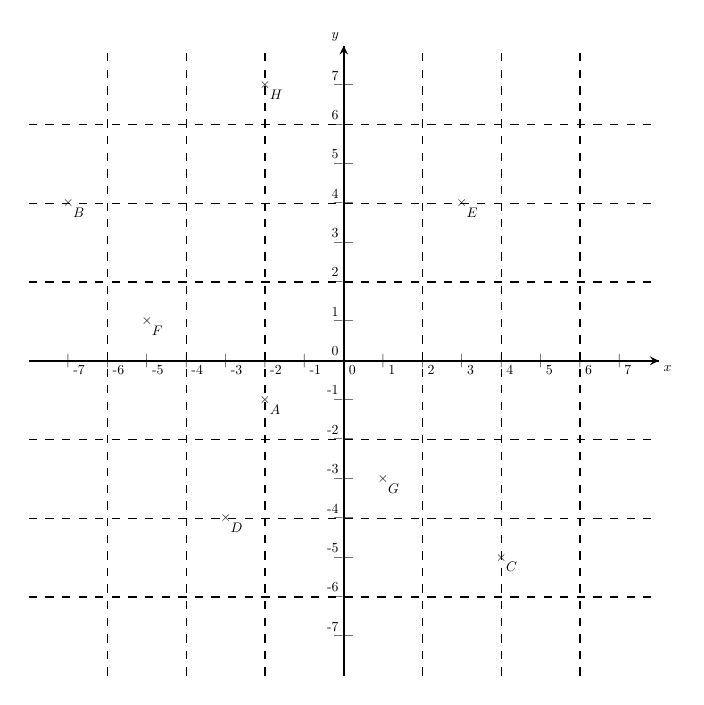
\begin{tikzpicture}[scale=0.5,every node/.style={scale=0.5}]
		%Points
		\coordinate(O)at(0,0);
		\coordinate(I)at(1,0);
		\coordinate(J)at(0,1);
		\coordinate(xstart)at(-8,0);
		\coordinate(xend)at(8,0);
		\coordinate(ystart)at(0,-8);
		\coordinate(yend)at(0,8);
		\coordinate(A)at(-2,-1);
		\coordinate(B)at(-7,4);
		\coordinate(C)at(4,-5);
		\coordinate(D)at(-3,-4);
		\coordinate(E)at(3,4);
		\coordinate(F)at(-5,1);
		\coordinate(G)at(1,-3);
		\coordinate(H)at(-2,7);
		%Étiquettes
	%	\draw (I) node[below right] {$1$};
	%	\draw (J) node[above left] {$1$};
		\draw (xend) node[below right] {$x$};
		\draw (yend) node[above left] {$y$};	
		%%%%%%%%%%%%%%%%%%%%%%%%%%%%%%%%%%%%
		%Axes
		\draw [thick] (xstart) -- (xend);
		\draw [thick] (ystart) -- (yend);
		%Flèches
	%	\draw [>=stealth,->] (O) -- (I);
	%	\draw [>=stealth,->] (O) -- (J);
		\draw [>=stealth,->] (O) -- (xend);
		\draw [>=stealth,->] (O) -- (yend);
	%	%Grille
	%	\draw [thin] (-8,-8)grid(8,8);
		%%%%%%%%%%%%%%%%%%%%%%%%%%%%%%%%%%%%
		%étiquettes
		\foreach \point in {A, ..., H}
			\draw(\point)node{$\times$};
		\foreach \point in {A, ..., H}
			\draw(\point)node[below right]{$\point$};		
		\foreach \r in {-7, -6, ..., 7}
	    	\draw[thick, below right] (\r,0) node{\r};
		\foreach \r in {-7, -6, ..., 7}
	    	\draw[thick, above left] (0,\r) node{\r};  
		\foreach \r in {-7, -6, ..., 7}
	    	\draw[thick] (\r,0) node{$|$};
		\foreach \r in {-7, -6, ..., 7}
	    	\draw[thick] (0,\r) node{$--$};
	   	\foreach \r in {-6, -4, ..., 6}
	    	\draw[dashed] (-8,\r)--(8,\r);
	   	\foreach \r in {-6, -4, ..., 6}
	    	\draw[dashed] (\r,-8)--(\r,8);
	%	\foreach \r in {0, 1,...,7}
	%    	\draw[thick, below right] (\r,0) node{\r};
	\end{tikzpicture}

\end{minipage}
\begin{minipage}{0.1\textwidth}
	\begin{enumerate}[]
		\item $\pointcoord{A}{~~~~}{~~~~}$
		\item $\pointcoord{B}{~~~~}{~~~~}$
		\item $\pointcoord{C}{~~~~}{~~~~}$
		\item $\pointcoord{D}{~~~~}{~~~~}$
		\item $\pointcoord{E}{~~~~}{~~~~}$
		\item $\pointcoord{F}{~~~~}{~~~~}$
		\item $\pointcoord{G}{~~~~}{~~~~}$
		\item $\pointcoord{H}{~~~~}{~~~~}$
	\end{enumerate}
\end{minipage}

\vspace{2em}

\begin{minipage}{0.35\textwidth}
				\begin{tikzpicture}[line cap=round,line join=round,>=triangle 45,x=1.0cm,y=1.0cm,scale=1,every node/.style={scale=1}]
			
			\tikzstyle{tiret}=[dash pattern=on 3pt off 3pt];
			\tikzstyle{domaine}=[domain=-5:8];
			\clip(-3.5,-2.5) rectangle (5.5,2.5);
			\draw [domaine] plot(\x,{(-0-0*\x)/1});
			\draw [domaine] plot(\x,{(-0--1*\x)/1});
			\draw [tiret,domaine] plot(\x,{(-1--1*\x)/1});
			\draw [tiret,domaine] plot(\x,{(-2--1*\x)/1});
			\draw [tiret,domaine] plot(\x,{(-3--1*\x)/1});
			\draw [tiret,domaine] plot(\x,{(-4--1*\x)/1});
			\draw [tiret,domaine] plot(\x,{(-5--1*\x)/1});
			\draw [tiret,domaine] plot(\x,{(--1--1*\x)/1});
			\draw [tiret,domaine] plot(\x,{(--2--1*\x)/1});
			\draw [tiret,domaine] plot(\x,{(--3--1*\x)/1});
			\draw [tiret,domaine] plot(\x,{(--1-0*\x)/1});
			\draw [tiret,domaine] plot(\x,{(--2-0*\x)/1});
			\draw [tiret,domaine] plot(\x,{(-1-0*\x)/1});
			\draw [tiret,domaine] plot(\x,{(-2-0*\x)/1});
			\draw [tiret,domaine] plot(\x,{(--4--1*\x)/1});
			\draw [tiret,domaine] plot(\x,{(-6--1*\x)/1});
			\draw [domaine] plot(\x,{(-0-0*\x)/-1});
			\draw [domaine] plot(\x,{(-0-0*\x)/-1});
			\draw [domaine] plot(\x,{(-0-0*\x)/-1});
			\begin{scriptsize}
			\draw (0,0) node {$\times$} node[above left] {$A$};
			\draw (1,0) node {$\times$} node[above left] {$I$};
			\draw (1,1) node {$\times$} node[above left] {$J$};
			\draw (3,0) node {$\times$} node[above left] {$E$};
			\draw (5,2) node {$\times$} node[above left] {$F$};
			\draw (1,-1) node {$\times$} node[above left] {$D$};
			\draw (-2,-2) node {$\times$} node[above left] {$C$};
			\draw (-2,2) node {$\times$} node[above left] {$B$};
			\draw (-3,0) node {$\times$} node[above left] {$G$};
			\draw (-3,-1) node {$\times$} node[above left] {$H$};
			\end{scriptsize}
			\end{tikzpicture}

\end{minipage}
\begin{minipage}{0.1\textwidth}
	\begin{enumerate}[]
		\item $\pointcoord{A}{~~~~}{~~~~}$
		\item $\pointcoord{B}{~~~~}{~~~~}$
		\item $\pointcoord{C}{~~~~}{~~~~}$
		\item $\pointcoord{D}{~~~~}{~~~~}$
		\item $\pointcoord{E}{~~~~}{~~~~}$
		\item $\pointcoord{F}{~~~~}{~~~~}$
		\item $\pointcoord{G}{~~~~}{~~~~}$
		\item $\pointcoord{H}{~~~~}{~~~~}$
	\end{enumerate}
\end{minipage}

